\documentclass[aps,twocolumn,secnumarabic,balancelastpage,amsmath,amssymb,nofootinbib, floatfix]{revtex4-2}

%%%%%%%%%%%%%%%%%%%%%%%%%%%%%%%%%%%%%%%%%%%%%%%%%%%%%%%%%%%%%%%%%%%

\usepackage{float}
\usepackage{graphicx}      % tools for importing graphics
%\usepackage{lgrind}        % convert program code listings to a form 
% includable in a LaTeX document
%\usepackage{xcolor}        % produces boxes or entire pages with 
% colored backgrounds
%\usepackage{longtable}     % helps with long table options
%\usepackage{epsf}          % old package handles encapsulated postscript issues
\usepackage{bm}            % special bold-math package. usge: \bm{mathsymbol}
\usepackage{siunitx}
%\usepackage{asymptote}     % For typesetting of mathematical illustrations
%\usepackage{thumbpdf}
\raggedbottom
\usepackage[colorlinks=true]{hyperref}  % this package should be added after 
% all others.
% usage: \url{http://web.mit.edu/8.13}


%%%%%%%%%%%%%%%%%%%%%%%%%%%%%%%%%%%%%%%%%%%%%%%%%%%%%%%%%%%%%%%%%%%
% And now, begin the document...
%%%%%%%%%%%%%%%%%%%%%%%%%%%%%%%%%%%%%%%%%%%%%%%%%%%%%%%%%%%%%%%%%%%

\begin{document}
	\title{Finding the Electron Rest Mass and Validating Special Relativity}
	\author{Octavio Vega}
	\email{ovega84@mit.edu}
	%\homepage{http://web.mit.edu/8.13/} %If you don't have one, just comment out this line.
	\date{\today}
	\affiliation{MIT Department of Physics}
	
	\begin{abstract}
		In this experiment, we observe the dynamics of relativistic particles and seek to determine two things: the rest mass of an electron, and whether special relativity provides a better model for kinetic energy than classical mechanics. We investigate the relationship between the electron's kinetic energy and its velocity inside a magnetic field after decay from a radioactive source. We measure energy spectra of detected electrons emerging from the radioactive decay of $^{90}Sr$. After determining the kinetic energy of the electrons in six different magnetic fields, we consider a linear relationship between their energies and their relativistic gamma factors in each scenario. The slope of this line, determined via linear regression, leads us to the value of $m_{e}c^{2}$. We compute a final value of $m_{e}c^{2}=\left(0.563\pm 0.013\pm 0.027\right)$ MeV, where the uncertainties are statistical and systematic, respectively.
	\end{abstract}
	
	\maketitle
	
	
	%%%%%%%%%%%%%%%%%%%%%%%%%%%%%%%%%%%%%%%%%%%%%%%%%%%%%%%%%%%%%%%%%%%%%%%%
	\section{Background and Relevant Theory}
	
	\subsection{History}
	Charged particles are often some of the smallest and most energetic particles in the universe, given that they exist at miniscule length scales on the order of angstroms ($\si{\angstrom}$) and travel at extremely high speeds nearing the speed of light $c$. 
	
	Reconciling Newtonian mechanics with Maxwell's theory of electromagnetism became a problem of the ages in the early 1900s. The challenge to find a broader model of physical dynamics beyond classical mechanics was revolutionized when the young Albert Einstein published his theory of "the electrodynamics of moving bodies," eventually known as special relativity. 
	
	In this experiment, we put to the test the framework of special relativity in the dynamics of electrons inside electric and magnetic fields, and seek to find our own answer to the contest between relativistic and classical models. 
	
	\subsection{Useful Electromagnetic Equations}
	The Lorentz force law gives the total force on a charged particle moving in the presence of an electric field $\vec{E}$ and a magnetic field $\vec{B}$:
	\begin{equation}\label{eq:lorentz}
		\vec{F} = q(\vec{E} + \vec{v} \times \vec{B})
	\end{equation}
	where the particle has charge $q$ and velocity $\vec{v}$. 
	Later on, we will see that inside a velocity selector, we can introduce an electric field such that the resulting force cancels the magnetic force; i.e. the net Lorentz force becomes zero such that
	\begin{equation}\label{eq:velocity}
		v=\frac{|\vec{E}|}{|\vec{B}|}
	\end{equation}
	
	It is also well known that the trajectories of moving charged particles are curved in the presence of magnetic fields. If the force on a charged particle is purely magnetic, then we can relate it to the centripetal force via the equation
	\begin{equation}\label{eq:centripetal}
		\frac{mv^{2}}{r}=qvB
	\end{equation}
	Solving equation~\ref{eq:centripetal} for the radius of the arc gives $r=\frac{mv}{qB}$.
	Making use of these relationships allows us to derive useful relations for the first major part of this experiment. 
	
	\subsection{Two Models for Energy}
	The second primary goal of this experiment is to investigate the relationship between kinetic energy and velocity; in particular, whether a relativistic or non-relativistic model describes this relationship better. Namely, the two relationships we investigate are given by 
	$$K(v)=\frac{1}{2}mv^{2}, \quad \text{for the non-relativistic model;}$$
	$$K(v)=mc^{2}(\gamma-1), \quad \text{for the relativistic model.}$$
		
	Note that the gamma factor we use throughout our analysis is given by $\gamma=(1-\frac{v^{2}}{c^{2}})^{-\frac{1}{2}}$, and the speed of light $c=299,792,458$ m/s is a fundamental constant we assume.
	
	\begin{figure}
		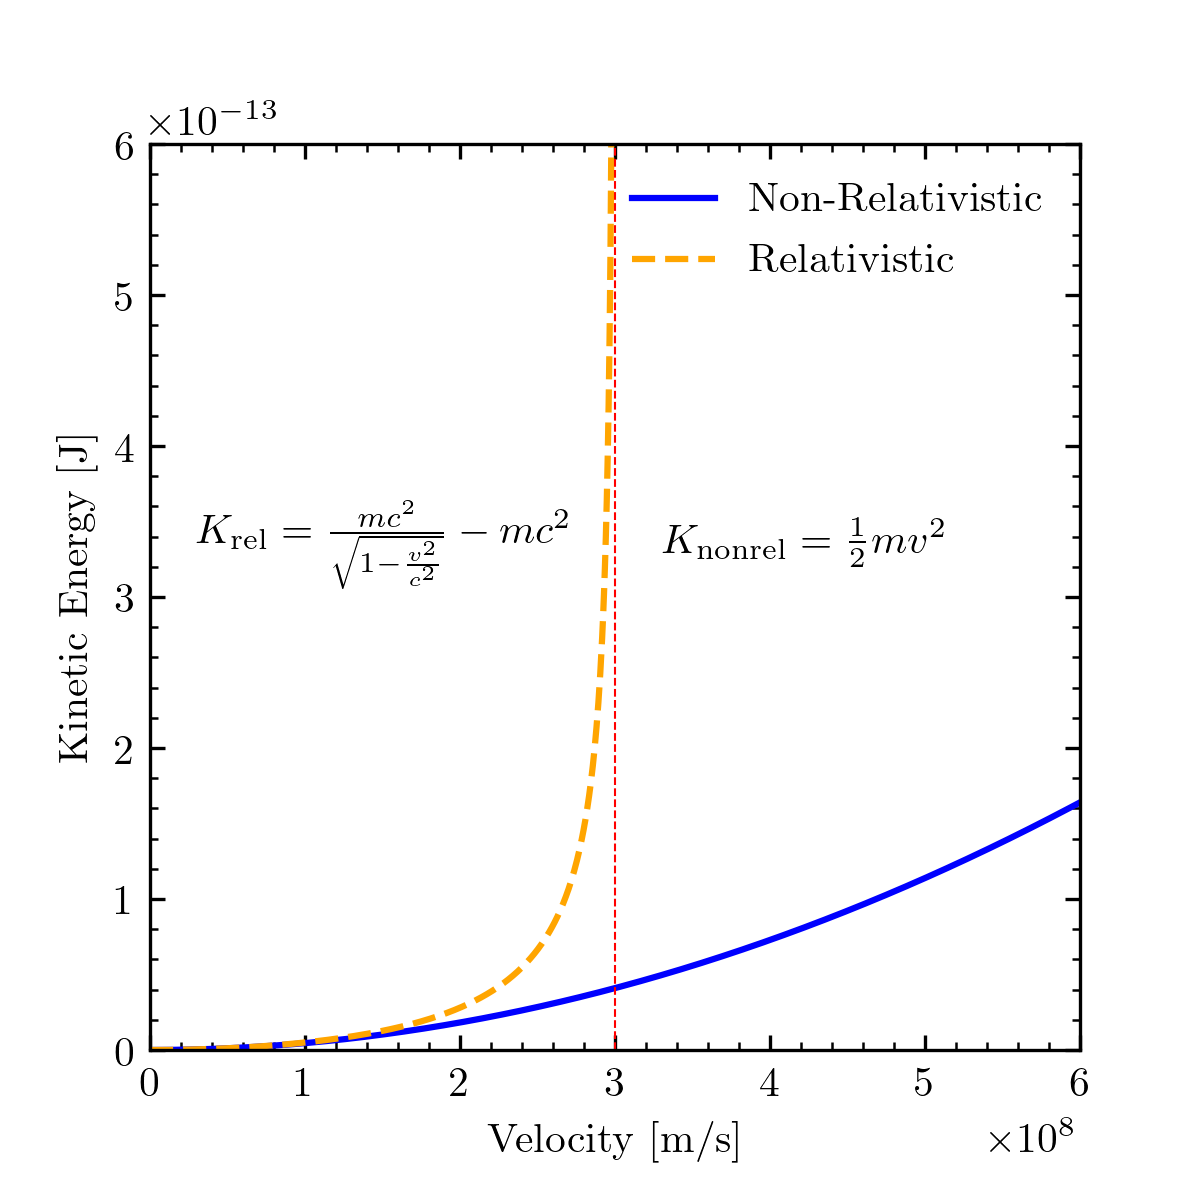
\includegraphics[width=9cm]{theoretical_ke_models.png}
		\caption{Theoretical models of kinetic energy as a function of velocity. The blue solid line depicts the non-relativistic model, while the orange dotted line illustrates the relativistic model.}
		\label{fig:model}
	\end{figure}
	
	Figure~\ref{fig:model} displays the comparison between the relativistic and non-relativistic models of kinetic energy as a function of velocity. I provide an example of what these theoretical models look like. 
	
	
	
	%%%%%%%%%%%%%%%%%%%%%%%%%%%%%%%%%%%%%%%%%%%%%%%%%%%%%%%%%%%%%%%%%%%%%%%%
	\section{Experimental Procedure}
	
	\begin{figure}[H]
		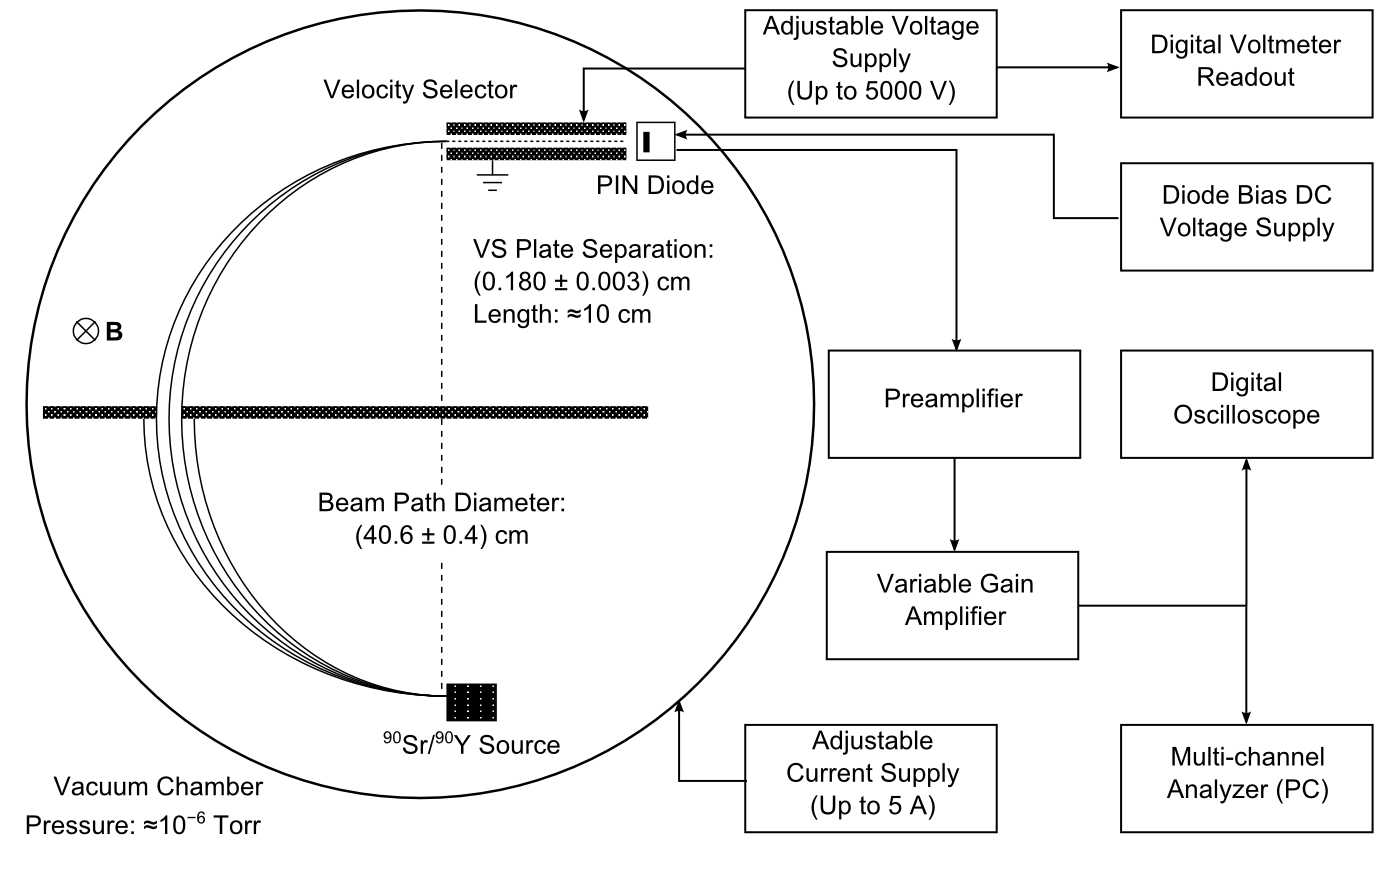
\includegraphics[width=9cm]{setup_block_diagram.png}
		\caption{A block diagram schematic of the main apparatus. Taken from the Junior Lab relativistic dynamics manual \cite{labmanual}}.
		\label{fig:apparat}
	\end{figure}
	
	Our apparatus consisted of the following components:
	\begin{itemize}
		\item Vacuum chamber: A large spherical orb wrapped in wire and connected to a current source. 
		\item Radioactive Source: For calibration, we insert a sample of $^{133}Ba$, and for the main experiment we use a sample of $^{90}Sr$. 
		\item Velocity Selector: Two plates between which there is a region of electric field that 'selects' particles of a particular velocity to proceed through, as per equation~\ref{eq:velocity}.
		\item Adjustable current supply: Provides current to the wire coils that wrap around the vacuum chamber, thereby generating a magnetic field of desired magnitutde inside. 
		\item Adjustable voltage supply: Generates an electric field across the plates of the velocity selector, intended to cancel the magnetic field. 
		\item PIN diode:  The PIN diode served as the particle detector, in which a detected electron registers as a voltage signal to be read.
		\item Amplifiers: The pre-amplifier and variable gain amplifier magnified the signals from the PIN diode to the MCA. Each day of data taking, we ensured that our amplifier settings were the same so that the resulting MCA spectrum would not be distorted. 
		\item Digital oscilloscope: The oscilloscope allows us to view the pulses arising from detected electrons in the PIN diode, serving as a check for indicating that a bin in the MCA was filled.
		\item Multi-channel Analyzer (MCA): The MCA was the primary data-gathering instrument, with which we collected histograms corresponding to the energy spectra in 2048 separate channels (bins). 
	\end{itemize}
	A diagram of the apparatus with the above components labeled is provided in Figure~\ref{fig:apparat}. 
	
	To determine stopping voltages, our procedure was as follows. We varied the input retarding voltage on the power supply incrementally up from 0 volts. After collecting numerous data points of retarding voltage versus photocurrent, we increased the retarding voltage until the resulting photocurrent was near zero nanoamps. At this point, we varied the retarding voltage around a small neighborhood of this point and determined the stopping voltage to within $\pm0.01$ volts.
	\subsection{Maximizing the Count Rate}
	We seek to set the voltage across the velocity selector such that the count rate the MCA records for each magnetic field value is maximized. To do so, we first collect data on the count rates for different velocity selector voltages at each value of magnetic field inside the vacuum chamber. For each $B$ field value, we test several voltages in increments of 0.1 kilovolts in a neighborhood of 4.5 kilovolts. 
	In figure~\ref{fig:countrate} I display the linear fit to the maximum count rate data. For the remainder of the experiment, we used this relationship to determine which voltage to set across the velocity selector at each $B$ field value.
	
	\begin{figure}[h]
		\centering
		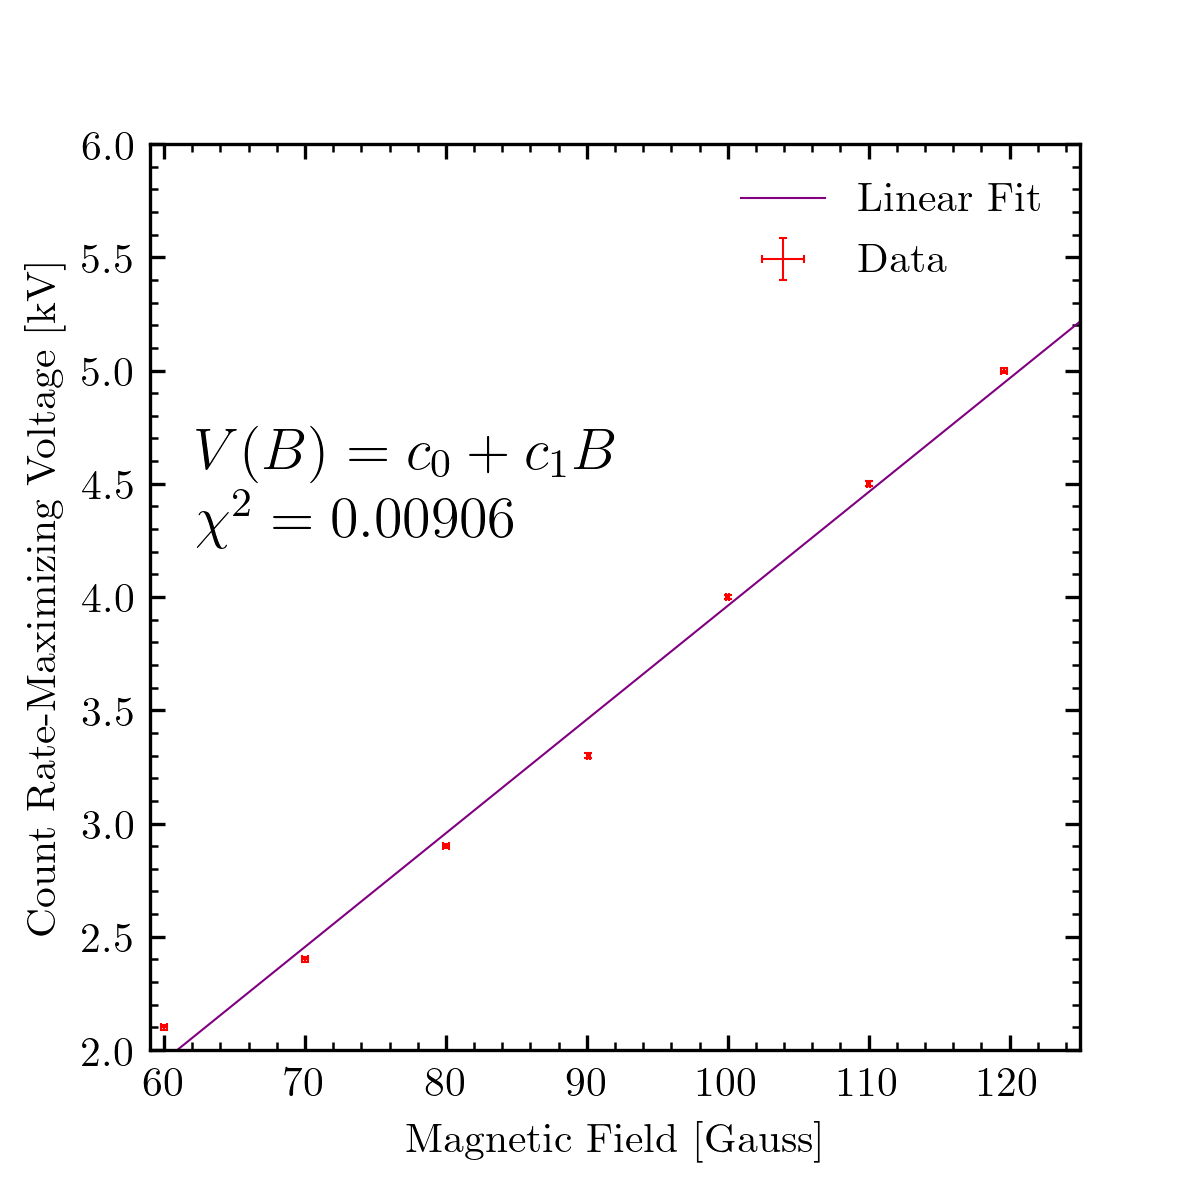
\includegraphics[width=9cm]{count_rate_max.png}
		\caption{The count rate data for each value of the $B$ field, with linear fit displayed.}
		\label{fig:countrate}
	\end{figure}
	
	\subsection{Calibrating the MCA}
	Each day of data taking, we calibrate the MCA with a sample of $^{133}Ba$ and comparing the observed energy spectrum to a known spectrum. On our first day of data collection, we allowed the MCA to collect data for approximately two hours. On subsequent days, we performed much shorter calibrations of about fifteen minutes each. 
	
	\begin{figure}[h]
		\centering
		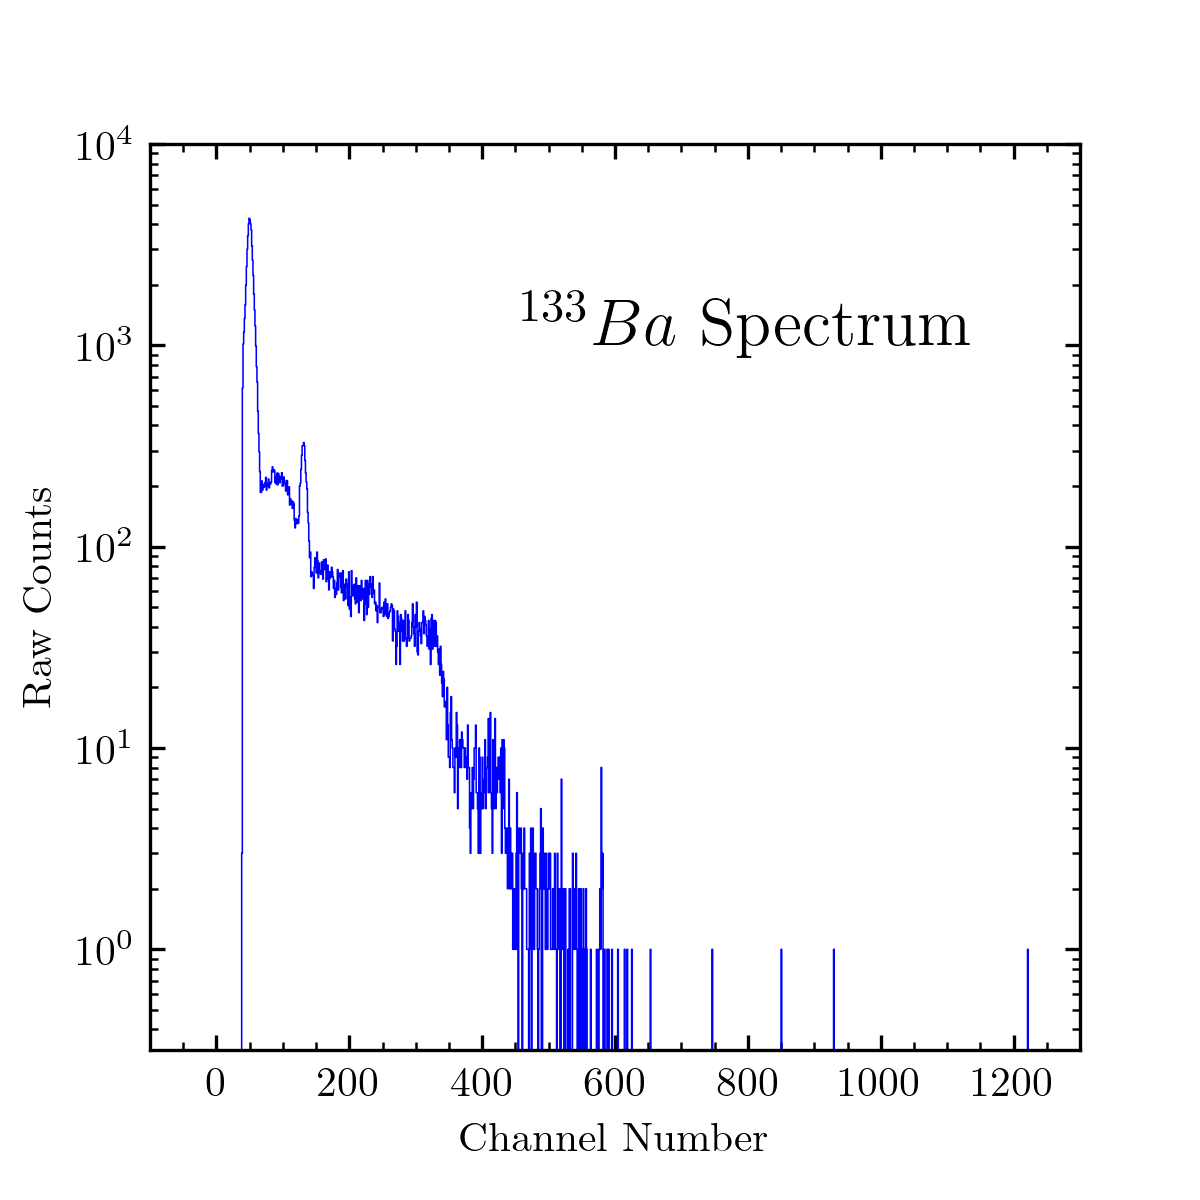
\includegraphics[width=9cm]{sample_calibration2.png}
		\caption{An example of one of our plots of the MCA output spectrum with uncalibrated bins on the x-axis simply corresponding to the channel number, and counts on the y-axis on a logarithmic scale.}
		\label{fig:calib}
	\end{figure}
	We compared the resulting spectrum from the $^{133}Ba$ decay to a known spectrum with peaks labelled by their corresponding energies. We matched our best guess of the peak energies to the corresponding MCA channel numbers we observed. From this data, we performed a linear fit to generate a linear relationship between the energies and channel numbers. We used this relationship to label our histogram bins by kinetic energy as opposed to channel number. In figure~\ref{fig:calib} I show an example of one such calibration spectrum with raw channel numbers and counts plotted on a logarithmic scale. 

	%%%%%%%%%%%%%%%%%%%%%%%%%%%%%%%%%%%%%%%%%%%%%%%%%%%%%%%%%%%%%%%
	\section{Data and Error Analysis}
	
	
	In this section I present raw data collected, as well as our reduced data followed by a discussion on the relevant errors and their sources. 
	
	\subsection{Raw Energy Spectra}
	
	For each of the six values for the internal magnetic field that we set, we record the energy spectrum that the MCA outputs and examine it for peaks. A peak corresponds to a most frequently detected energy value deposited into the detector. We fit a gaussian curve to each spectrum at the peak to determine the center of the peak, which we take to be the kinetic energy of the detected electron at each value of the $B$ field. 
	
	\begin{figure}
		\centering
		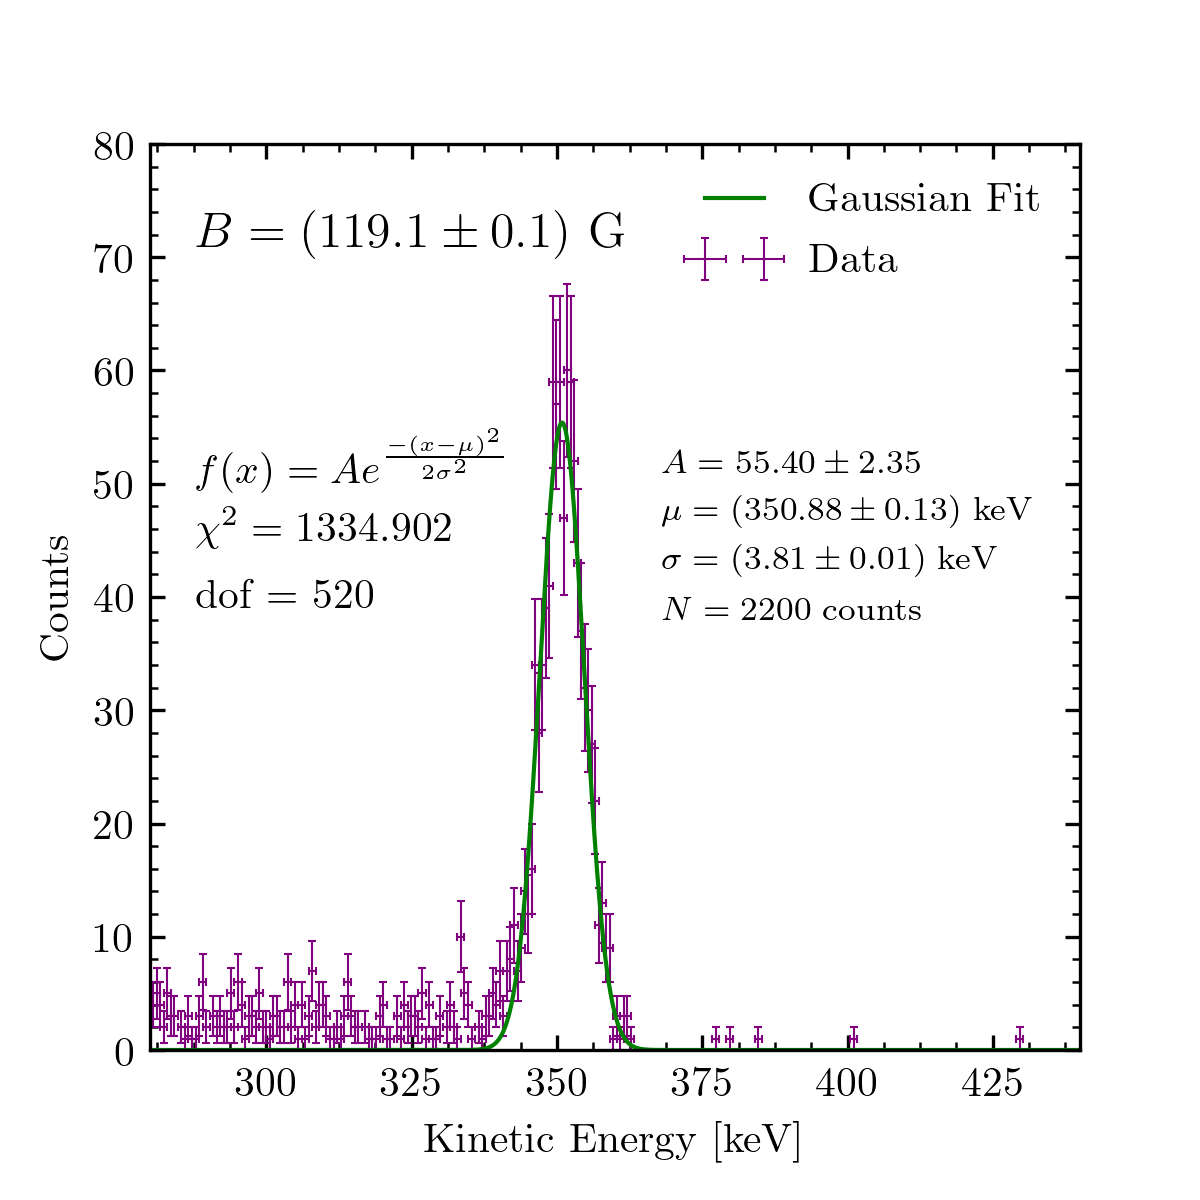
\includegraphics[width=9cm]{espectrum_b120.png}
		\caption{The peak in the raw spectrum of detected electron energies in the MCA at a magnetic field value of about 120 Gauss, overlaid on which is a gaussian curve fit to the peak.}
		\label{fig:espectrum}
	\end{figure}
	
	In figure~\ref{fig:espectrum} I plot the raw data for the energy spectrum along with the best fit gaussian function, and display the best-fit parameters with corresponding standard uncertainties.
	
	\subsection{Fitting to the Rest Energy} 
	
	After determining the electron kinetic energies for each of the six magnetic field values, I plot the kinetic energies against the gamma factor $\gamma(v)$ in each scenario in figure~\ref{fig:restmassfit}.
	
	\begin{figure}
		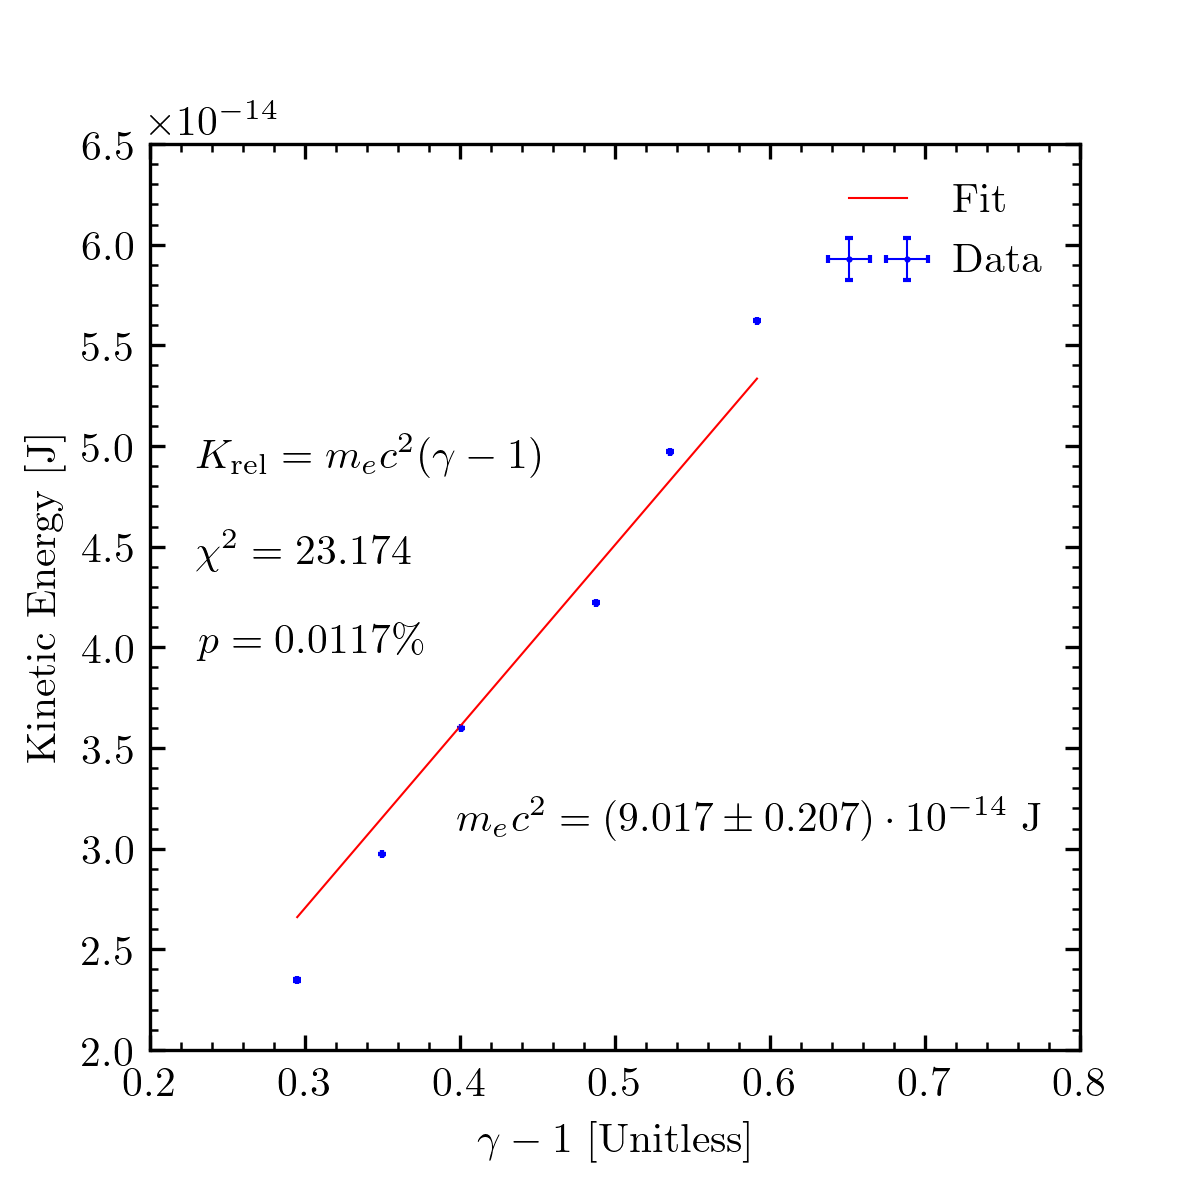
\includegraphics[width=9cm]{k_vs_gamma.png}
		\caption{A linear regression model fit to the kinetic energy vs. gamma factor data. The slope of the linear curve is equal to the rest mass of the electron, i.e. $m_{e}c^{2}$.}
		\label{fig:restmassfit}
	\end{figure}
	
	
	I fit a linear function to the data, whose slope is given by the $m_{e}c^{2}$ and vertical intercept is fixed to be 0 by the functional form of the model assumed. Computing the best fit slope, I find a value for the electron's rest energy of $m_{e}c^{2}=(9.017\pm 0.207)\cdot 10^{-14}$ J.
	
	\subsection{Comparison of Kinetic Energy Models to Data}
	
	In order to fulfill the second goal of the experimental analysis, we recall that we have two models in contention for representing the kinetic energy as a function of velocity. To determine which is more valid, we fit the data to each of the two functional forms and perform a statistical goodness of fit test on both fits. 
	\begin{figure}
		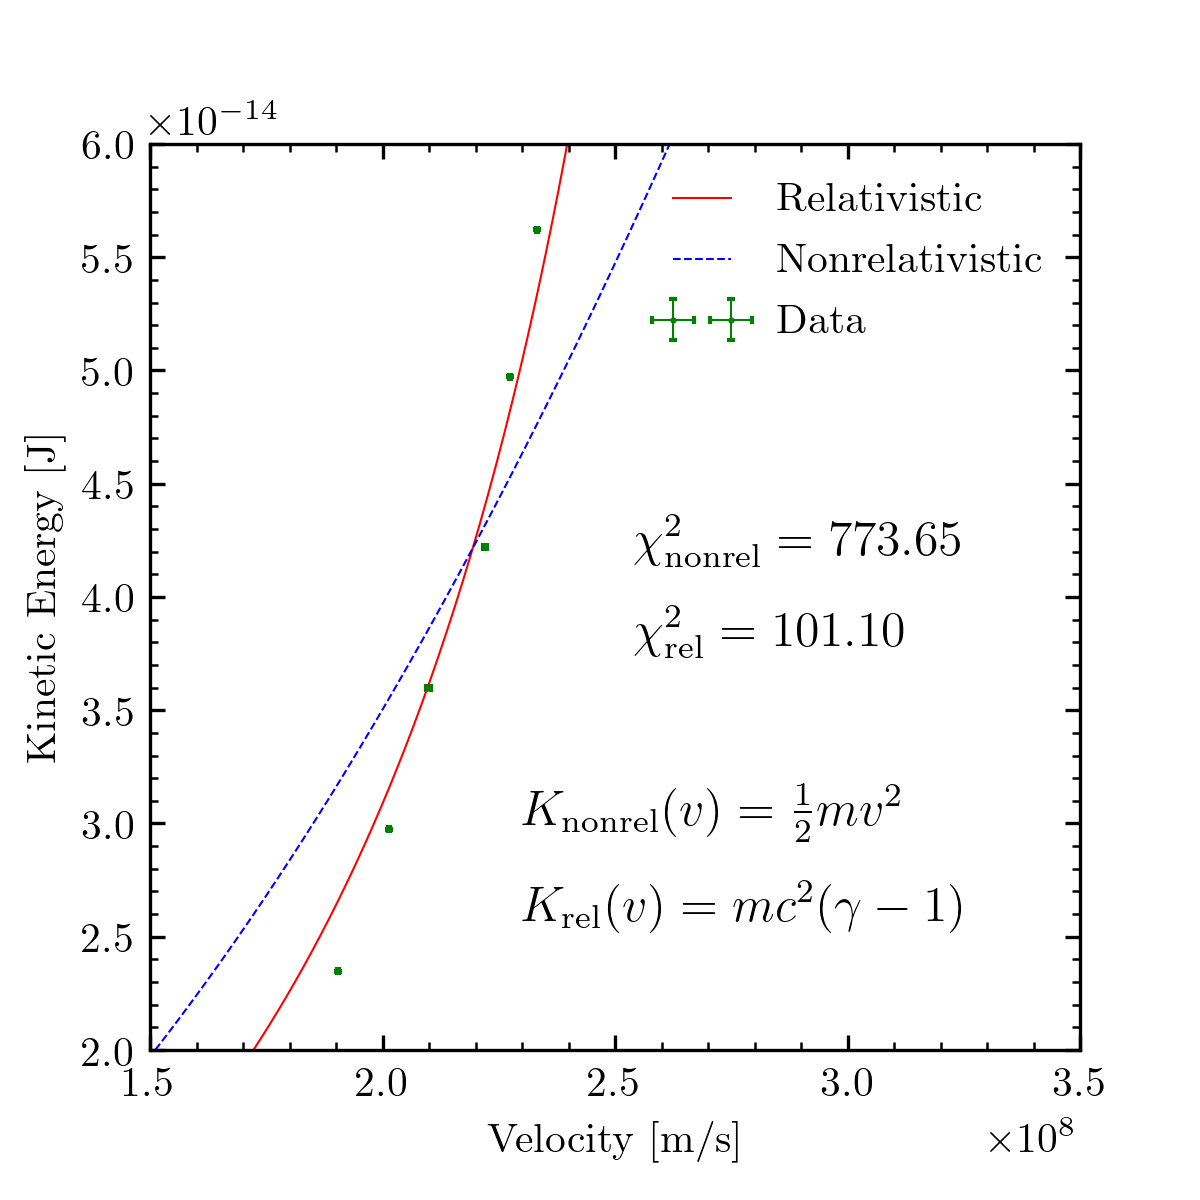
\includegraphics[width=9cm]{model_data_comparison.png}
		\caption{The data points for kinetic energy versus the corresponding velocities, over which both the relativistic and non-relativistic kinetic energy functions are superimposed.}
		\label{fig:modeldata}
	\end{figure}

	
	Figure~\ref{fig:modeldata} displays the kinetic energy data, as well as the two best fit curves for each of the models. The resulting $\chi^{2}$ values for each fit are displayed in the plot. We see that $\chi^{2}_{\text{rel}}<\chi^{2}_{\text{nonrel}}$, indicating that the relativistic function for kinetic energy $K(v)=mc^{2}[\gamma(v)-1]$ is a much better representation of the real data than the classical model.
	
	
	\subsection{Error Estimation and Discussion}
	I estimate the statistical uncertainties and systematic uncertainties in my measurement of $m_{e}c^{2}$ to be $2.309\%$ and $4.796\%$, respectively. 
	
	Due to the precision of the equipment used in this experiment, the statistical uncertainty is relatively low and contributes less to the total uncertainty of the measurement. Some contributors to the statistical uncertainty of my measurement include
	\begin{itemize}
		\item Lack of repeated trials: for each of the six $B$ field values, we only collected one electron energy spectrum in the MCA, and thereby only found one value of the kinetic energy for each trial. 
		\item We observed some fluctuations in the magnetic field inside our vacuum changer during data collecting, leading to higher uncertainties on our calculations for the velocities of the electrons, according to formula~\ref{eq:velocity}. 
	\end{itemize}
	
	I attribute the sources of the systematic uncertainty to a number of factors:
	\begin{itemize}
		\item We  encountered some variability in the amplifier settings beyond our control; in earlier trials, we discovered more than one peak emerging in our MCA spectrum, indicating that the amplification of each signal was shifting back and forth between two values. While we switched amplifiers thereafter, we are still uncertain as to the cause of this and whether it impacted our more recent trials. 
		\item The gaussian functional form used to fit the electron energy spectra may not have been the best model to use; i.e. there is cause to have included an additional background term of perhaps linear or polynomial order, or to include another gaussian since the signal is the result of two decay processes happening in succession. 
	\end{itemize}  
	
	
	%%%%%%%%%%%%%%%%%%%%%%%%%%%%%%%%%%%%%%%%%%%%%%%%%%%%%%%%%%%%%%
	\section{Conclusions}
	Our final result for the electron rest energy is $m_{e}c^{2}=(0.563\pm0.013_{\text{stat}}\pm0.027_{\text{sys}})$ MeV. Hence, we ultimately compute a value for $m_{e}c^{2}$ to within 10\% of the true value, which is 0.5110 MeV as documented in literature. Furthermore, our we confirm that the relativistic framework for conceptualizing kinetic energy as a function of velocity is superior to the classical model. 
	
	The accuracy of our result might improve with more strict observation of sources of systematic uncertainty. With better time budgeting, we would perform multiple trials at each step of our experiment to reduce standard errors; for instance, if we were to repeat this experiment with more time, we would perform several measurements of the electron energy spectrum at each $B$ field value, as opposed to a single measurement. 
	
	Nonetheless, we take our results as indicative of not only well-documented physics thus far but also of future tests to probe the fabric of the standard model of physics. The radioactive decays we leverage in this experiment are themselves mediated by the weak force, given that electron antineutrinos $\bar{\nu}_{e}$ are emitted as well. As standard model particles, neutrinos are elusive and difficult to detect but our experimental results suggest that with much larger scale and higher energy particle detectors, the electroweak unification of quantum field theory is subject to probing \cite{neutrinos}. 
	
	
	%%%%%%%%%%%%%%%%%%%%%%%%%%%%%%%%%%%%%%%%%%%%%%%%%%%%%%%%%%%%%%%%%%%%%%%
	\begin{acknowledgments} The author is very grateful to Luke Gianni for serving as his lab partner throughout this experiment. The author is also very thankful for the constructive feedback offered by Professor Fakhri. The author would additionally like to thank Hanzhen Lin for their useful discussions on various related topics. 
	\end{acknowledgments}
	
	%%%%%%%%%%%%%%%%%%%%%%%%%%%%%%%%%%%%%%%%%%%%%%%%%%%%%%%%%%%%%%%%%%%%%%%%% 
	
	\bibliography{paper1}
	
\end{document}
